\section{Comparaison and Application to RTI Fields}

\subsection{Comparaison Criteria}
In the context of this work, the main criteria for comparing Fourier and wavelet representations are the number of coefficients required to accurately reconstruct the signal, the ability to capture localized structures and sharp gradients, the effectiveness of separating structures across different scales, and the generalization capabilities to unseen data or different flow regimes. Figure \ref{fig:representation_comparison} illustrates the reconstruction of a two-dimensional Rayleigh--Taylor density field using Fourier, wavelet, and PCA representations with the same number of coefficients. The comparison highlights the differences in capturing sharp gradients and gibbs-like oscillations.
It is also important to note that the PCA is used here as a reference for comparison, but it is not a practical solution for generative modeling since it requires access to the entire training dataset and does not provide extrapolation capabilities for unseen samples.

\begin{figure}[h]
\centering
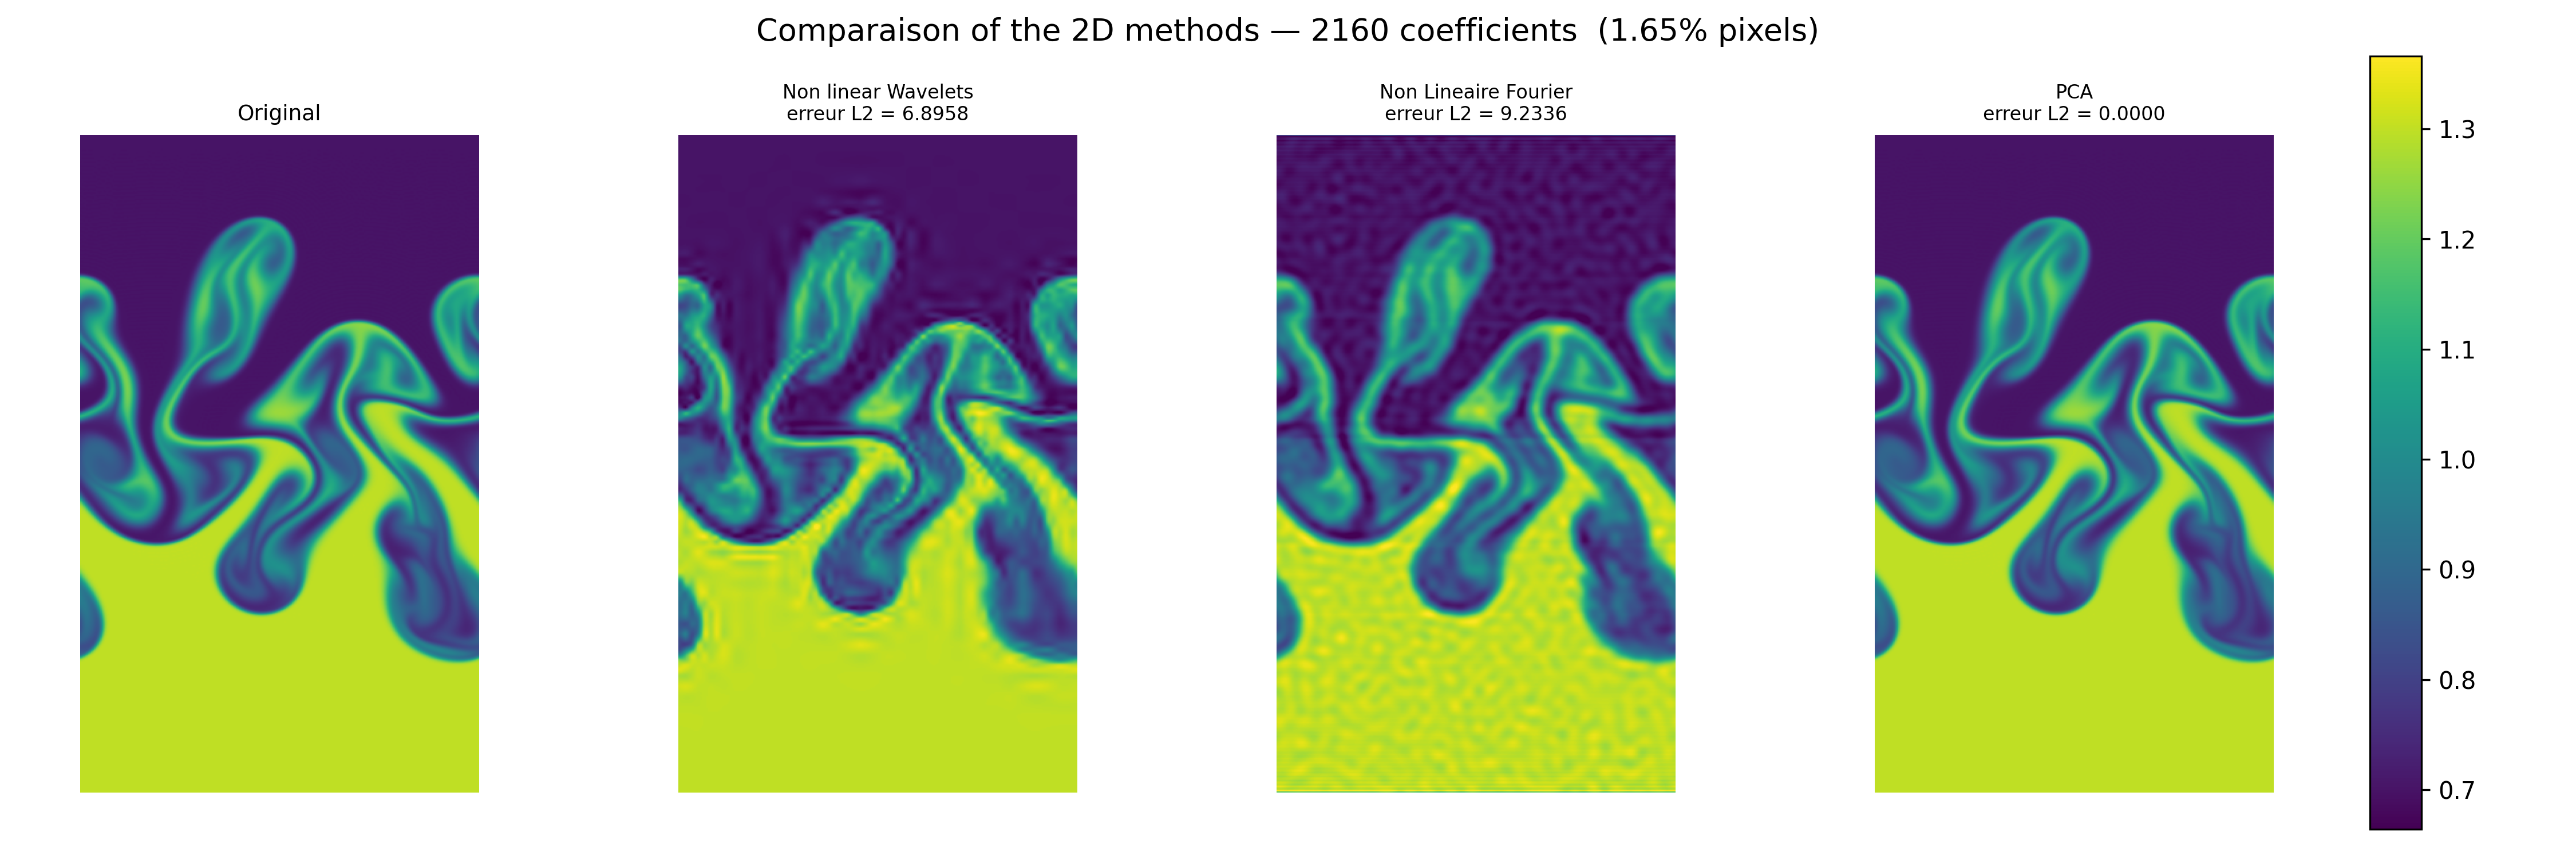
\includegraphics[width=0.9\textwidth]{figures/ch2/Verification_zone_melange.png}
\caption{Comparison of different representations for a two-dimensional Rayleigh--Taylor density field}
\label{fig:representation_comparison}
\end{figure}

For more quantitative comparisons, the reconstruction error is computed as the L2 norm between the original field and its reconstruction. Figure \ref{fig:representation_error_comparison} shows the evolution of the reconstruction error as a function of the number of coefficients for Fourier, wavelet, and PCA representations. The results indicate that wavelet representations generally provide better reconstruction after a certain number of coefficients having a very steep decrease of the error.

\begin{figure}[h]
\centering
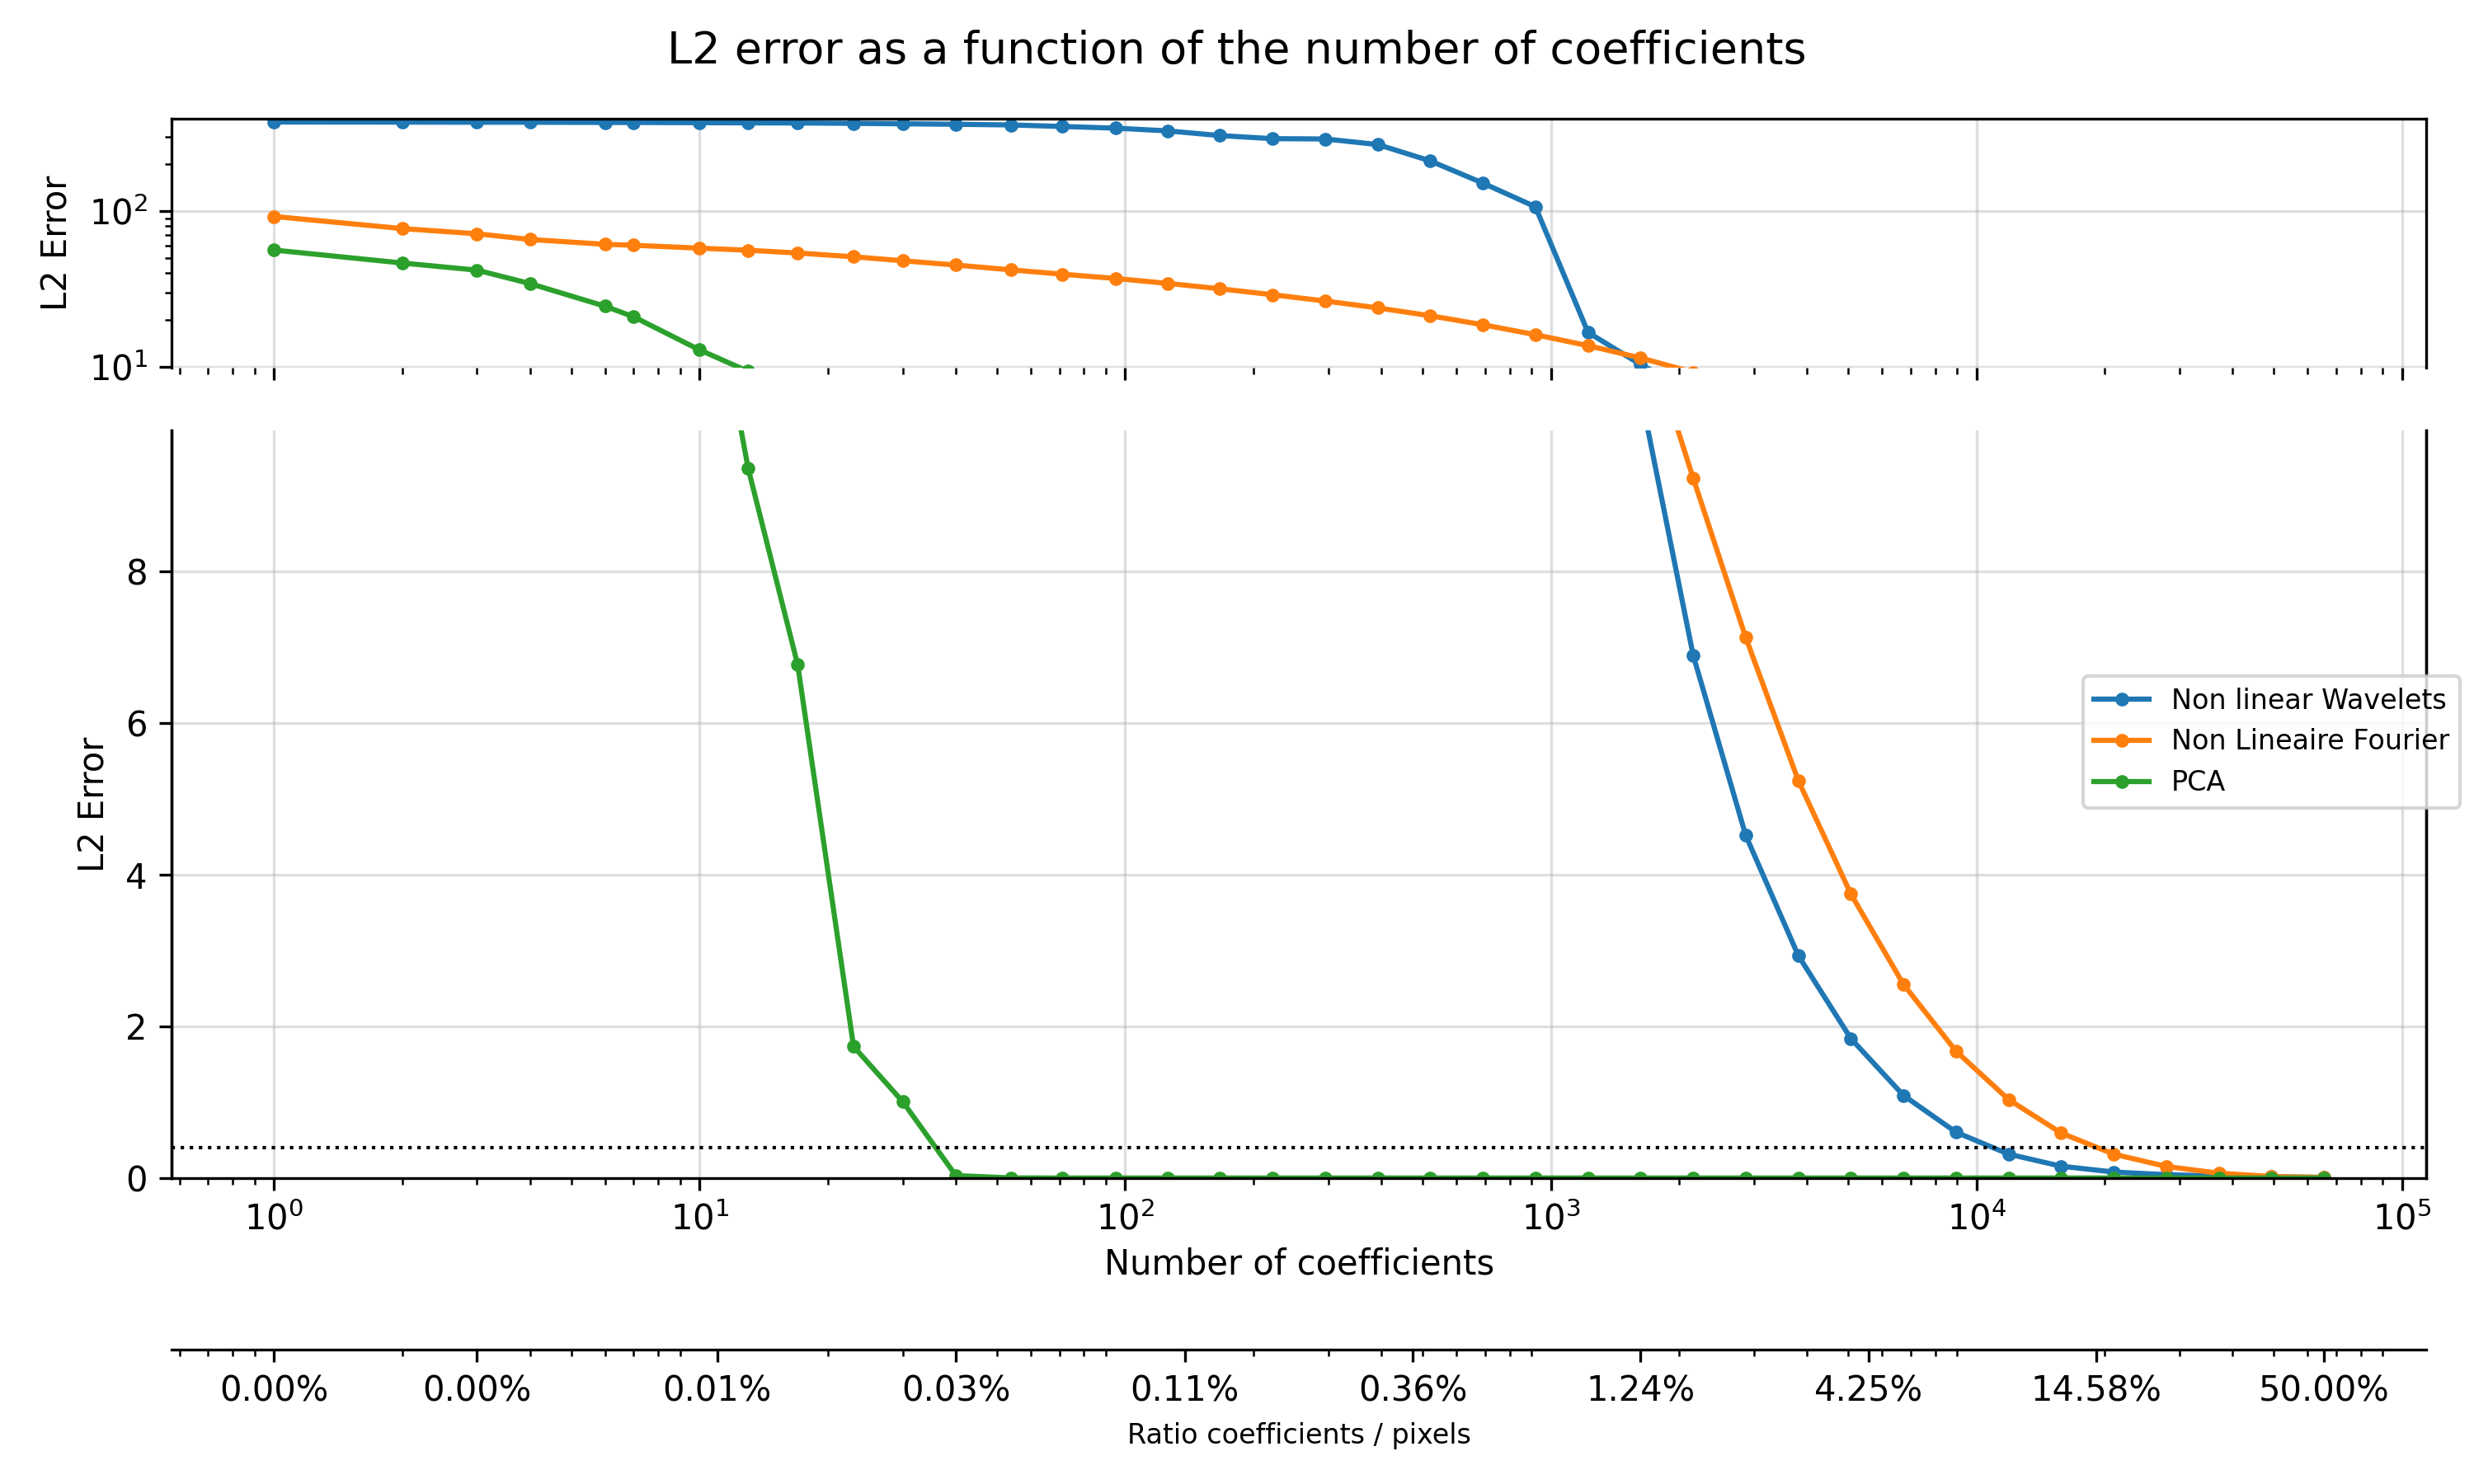
\includegraphics[width=0.65\textwidth]{figures/ch2/dataset2D_Comparaison_des_Erreurs.png}
\caption{Comparison of different representations for a two-dimensional Rayleigh--Taylor density field}
\label{fig:representation_error_comparison}
\end{figure}

With the same number of coefficients, wavelet representations generally provide better reconstruction of localized structures and sharp gradients compared to Fourier representations. It is for sure less performing than PCA, but it is more robust and independent of the training dataset. The multi-scale nature of wavelet decompositions also allows for a more natural separation of structures across different scales, which is particularly relevant for turbulent RTI flows.
